\documentclass{beamer}
\usepackage{amsmath}

\usetheme{boxes}

\usepackage{Sweave}
\begin{document}
\Sconcordance{concordance:moz-model-pres.tex:moz-model-pres.Rnw:%
1 14 1 1 0 25 1 1 13 1 2 267 1}

\title{Slightly Less Simple Mosquito Modeling}
\author[Pearson]{Carl~A.~B.~Pearson}
\institute[University of Florida]{
Emerging Pathogens Institute, University of Florida
}
\frame{\titlepage}

\frame{

\begin{figure}
\begin{center}
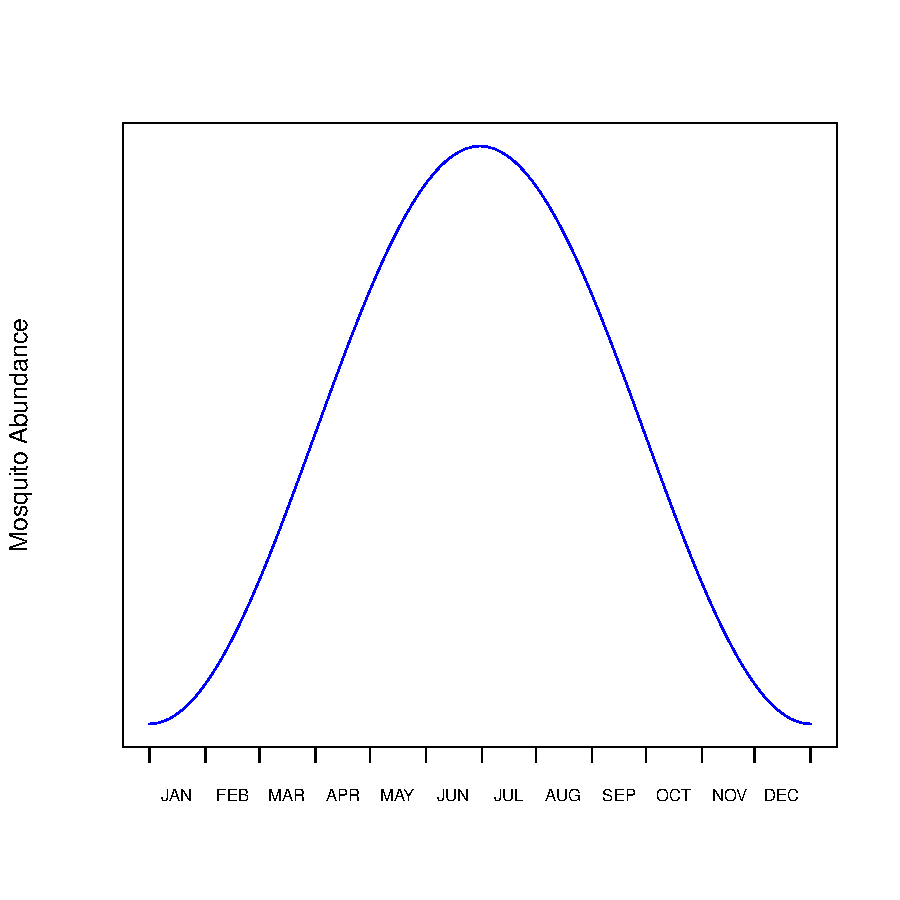
\includegraphics{moz-model-pres-plotfig1}
\end{center}
\end{figure}

}

\frame{

\begin{figure}
\begin{center}
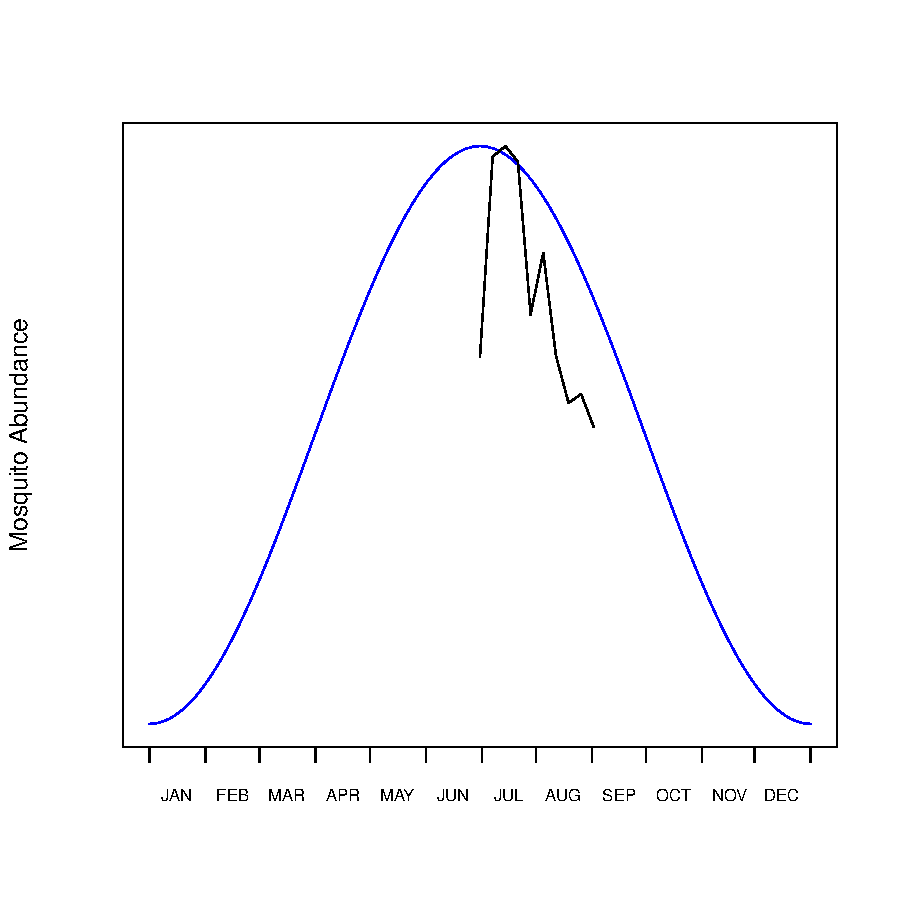
\includegraphics{moz-model-pres-plotfig2}
\end{center}
\end{figure}

}

\frame{
\frametitle{Emphasis: Simple}
comparison of continuous, spatially homogenous models

Why? 

understanding of infection trends can inform interventions, health system preparations, {\em etc}.
}

\frame{
\frametitle{Common Mosquito Model} % in disease contexts, not used absolutely everywhere

TODO sine
}

\frame{
\frametitle{...{\em vs.} Common Mosquito Abundance}

TODO overlay mosquito pops with sine, match peaks
}

\frame{
\frametitle{So, Low Hanging Fruit}

preview: no sophisticated analysis to pick said fruit \\
but these basic analyses provide fertile ground for much more quantitative detail
% note about the value of this approach in general to science engineering
}

\frame{
\title{Engineering \&\ Maths Refresher, I}
\begin{enumerate}
\item useful to write models in terms of measurable parameters,
\item measurable parameters are not scale-free,
\item mathematics is more useful when scale free, therefore
\item dimensional analysis is awesome
\end{enumerate}
}

% \frame{
% where $M(t)$ is mosquito population w.r.t time
% \begin{align*}
% \dot{M(t)} = E(t) - \lambda M(t)
% \end{align*}
% defined on $t\in(-T/2,T/2)$
% }
% 
% \frame{
% common usage is $M(t)\propto$ simple trigonometric
% 
% What salient observed features does that miss?
% 
% aside: why replace given $M(t)$ with given $\dot{M(t)}$?
% }
% 
% \frame{
% Salient features:
% \begin{itemize}
% \item short time with appreciable population
% % note: measure of pop. may be totally unreliable; however, trappable pop might good surrogate for active pop.
% \item even shorter time for population rise and fall
% \item low correlation with early and peak populations % accurate? provide comparison plots?
% \end{itemize}
% 
% Need a spike-like $E(t)$ to replicate these.  Candidates?
% }
% 
% \frame{
% Spike-like could be more formally $\delta$-function like.
% 
% So: use $\delta$-function approximations.
% }
% 
% \frame{
% TODO list approximate delta functions.
% }
% 
% \frame{
% What should we use for the shape parameters?
% 
% clue: want oranges-to-oranges comparisons between the options
% }
% 
% \frame{
% I chose to make mosquito total births equivalent
% 
% TODO $M_p$ equation
% 
% and then to apply a subjective ``constraint'' on $\Delta t$
% 
% TODO delta t stuff
% }
% 
% \frame{
% TODO list approximate delta functions with params in place
% }
% 
% \frame{
% Now everything is on the same scale, but rewind: don't have any of the convenience of having the same scale.
% 
% So: dimensional analysis.  What parameters should be eliminated?
% }

\end{document}
